\chapter{Alineación de imágenes}
\label{capitulo4}
\lhead{Capítulo 4. \emph{Alineación de imágenes}}

\section{Introducción}

En la sección anterior se estudió la primera etapa del proceso de registro de imágenes, estableciendo la correspondencia de puntos entre estas. En la presente se describe la etapa de registro pero abordando el tema de las transformaciones geométricas, en primer lugar presentando una descripción y explicación de su estructura y seguido del proceso de su estimación a partir de los puntos previamente obtenidos. Una vez la etapa de registro este completa, se profundiza en el proceso para la alineación de imágenes en un plano común, presentando los algoritmos utilizados para su implementación, así como también técnicas para reducir el error acumulado de las etapas anteriores. Finalmente se presentan resultados por separado de cada proceso previamente descrito, con su respectivo análisis.

\section{Revisión teórica}

A continuación se expone una revisión de los conceptos básicos que involucran una transformación geométrica, donde se plantea una jerarquía de los distintos niveles de transformaciones basadas en sus propiedades geométricas. Una vez se tengan claros estos conceptos, se presentan los métodos matemáticos que permiten obtener dichas transformaciones. 

\subsection{Transformaciones geométricas}

El siguiente paso en el proceso de registro, luego de establecer la correspondencia entre las imágenes, es encontrar la transformación geométrica que permite alinearlas. Para comprender su funcionamiento es necesario introducir el concepto de espacio proyectivo, sobre el cual se efectuarán dichas transformaciones. En base a esto comenzaremos presentando la convención de notación homogénea para puntos y lineas en este espacio.

Una linea en el espacio representada por la ecuación $ax + by + c = 0$, se puede expresar en forma vectorial de la forma $(a,\, b,\, c)$. Así, los vectores $k(a,\, b,\, c)$ representan todo el conjunto de rectas que son equivalentes --- $(ka)x + (kb)y + (k)c = 0$ ---, para cualquier $k\neq0$. De esta forma, se conoce como un vector homogéneo al vector particular que pertenezca a un grupo de vectores bajo esta relación de equivalencia. En base a este concepto se introduce la definición \ref{espacio-p} de espacio proyectivo.

\begin{displayquote}
	\vspace{-1.5cm}
	\begin{definition}
		El espacio proyectivo ${\rm I\!P}^2$ está conformado por el grupo de rectas o vectores equivalentes en el conjunto ${\rm I\!R}^2-\{0\}$, es decir, excluyendo la recta $(0,\, 0,\, 0)$.
		\label{espacio-p}
	\end{definition}
\end{displayquote}

Conociendo el espacio proyectivo y la notación de vectores homogéneos, procede a definir el concepto de puntos homogéneos, y establecer una relación que nos permita transformarlos a su espacio euclidiano original. 

Teniendo un punto $\vec{x}=(x,\, y)$, este pertenece a la recta $\vec{l}=(a,\, b,\, c)$ si logra satisfacer su ecuación --- $ax + by + c = 0$ ---. Si lo escribimos en forma vectorial, tendríamos $(x,\, y,\, 1)(a,\, b,\, c) = 0$, esto es añadiendo un 1 como tercer componente del punto $\vec{x}$. Similar al concepto previo de vectores homogéneos, se tiene que el conjunto de puntos $k(x,\, y,\, 1)$ son representaciones equivalentes del mismo punto, ya que todo ese conjunto pertenece a la misma recta --- $k(x,\, y,\, 1)(a,\, b,\, c) = 0 \to (ka)x + (kb)y + (k)c = 0$ ---. Así, añadiendo esta coordenada, tenemos que los puntos son representados como vectores homogéneos y pertenecen al espacio ${\rm I\!P}^2$. De esta forma se introduce la siguiente definición \ref{punto-homogeneo} que relaciona la siguiente conversión: ${\rm I\!P}^2 \to {\rm I\!R}^2$.
\begin{displayquote}
	\vspace{-1.5cm}
	\begin{definition}
		La representación de un vector homogéneo es de la forma $\vec{x} = (x_1,\, x_2,\, x_3)$, representando el punto $(x_1/x_3,\, x_2/x_3)$ en ${\rm I\!R}^2$, con $x_3 \neq 0$.
	\end{definition} 
	\label{punto-homogeneo}
\end{displayquote}

Teniendo claros los conceptos de representación homogénea, se presenta formalmente la definición de una homografía (\ref{def-homografia}) o transformación geométrica en el espacio proyectivo.
\begin{displayquote}
	\vspace{-1.5cm}
	\begin{theorem}
		Una transformación $h : {\rm I\!P}^2 \to {\rm I\!P}^2$ es una homografia si y solo si existe una matriz no singular $\vec{H}_{3x3}$, para la cual, cualquier punto en ${\rm I\!P}^2$ representado por un vector $\vec{x}$ se cumple que $h(\vec{x}) = \vec{H}\,\vec{x}$.
		\label{def-homografia}
	\end{theorem} 
\end{displayquote}

Existen varias formas de describir las transformaciones geométricas, la primera es algebraica, en la cual se muestra la estructura de la matriz de transformación, y la segunda es analizando las variables que se mantienen invariantes luego de aplicar dicha transformación. Adicionalmente, cada transformación geométrica está caracterizada por los grados de libertad, o la cantidad de parámetros que cada una puede variar sobre la imagen de entrada. Esta definición se introduce a continuación (\ref{def-dof}).
\begin{displayquote}
	\vspace{-1.5cm}
	\begin{definition}
		Los grados de libertad \textit{DoF} (del inglés: Degrees of Freedom), son la cantidad mínima de parámetros independientes que pueden especificar el movimiento de un objeto. En otras palabras, es la mínima cantidad de movimientos independientes que puede realizar un objeto. En el caso de transformaciones geométricas corresponde con el numero de componentes "libres" que permiten especificar dicha transformación.
		\label{def-dof}
	\end{definition} 
\end{displayquote}

En base a los grados de libertad, a las propiedades geométricas y al tipo de invarianza que presenten, se tienen cuatro niveles de transformaciones geométricas: isometría, similaridad, afín y perspectiva. Estos son descritos a continuación.
%${\rm I\!P}^2$, ${\rm I\!R}$ 
%%%%%%%%%%%%%%%%%%%%%%%%%%%%%%%%%%%%%%%%%%%%%%%%%%%%%%%%%%
\subsubsection*{ISOMETRÍA}

Este termino proviene del griego iso (igual) metria (medida), y tal como su nombre lo indica, ésta transformación se caracteriza fuertemente por mantener iguales las longitudes entre todos los puntos. Ésta se compone por una combinación de rotaciones y translaciones --- transformaciones euclidianas --- donde se modela el movimiento de un objeto rígido. En la ecuación \ref{matriz-isometria} se puede observar su representación matricial.

\begin{equation}
	\begin{pmatrix}
	{x'}\\{y'}\\{1}
	\end{pmatrix} = 
	\begin{bmatrix}
	{\cos \theta}&{-\sin \theta}&{tx}\\
	{\sin \theta}&{\cos \theta}&{ty}\\
	{0}&{0}&{1}
	\end{bmatrix}
	\begin{pmatrix}
	{x}\\{y}\\{1}
	\end{pmatrix}
	\label{matriz-isometria}
\end{equation}
\begin{displaymath}
(x', \,y', \,1) \to (x',\, y') 
\end{displaymath}
Esta matriz es posible expresarla por bloques, como se muestra a continuación:
\begin{displaymath}
\vec{x'}= 
\begin{bmatrix}
{\mathtt{R}}&{\vec{t}}\\
{\vec{0}}&{1}
\end{bmatrix}
\vec{x}
\label{bloque-isometria}
\end{displaymath}
Donde $ \mathtt{R} $ sería una matriz ortogonal de rotación $2\times2$, $ \vec{t} $ es un vector columna de translación de 2 componentes y $\vec{0} $ es un vector fila nulo de 2 componentes.
\begin{itemize}
	\item \textbf{Invarianza:} Distancia entre puntos, ángulo entre lineas y área.
	\item \textbf{3 Grados de libertad:} Ángulo de rotación, traslación en eje $x$, traslación en eje $y$. Puede ser calculada a partir de dos puntos correspondientes.
\end{itemize}

%%%%%%%%%%%%%%%%%%%%%%%%%%%%%%%%%%%%%%%%%%%%%%%%%%%%%%%%%%
\subsubsection*{SIMILARIDAD}

Esta transformación es una combinación de una isometría con un escalado, en este caso el escalado es de igual magnitud en los ejes $x$ e $y$. La representación matricial se observa en la ecuación \ref{matriz-similaridad}.

\begin{equation}
\begin{pmatrix}
{x'}\\{y'}\\{1}
\end{pmatrix} = 
\begin{bmatrix}
{s\, \cos \theta}&{-s\, \sin \theta}&{tx}\\
{s\, \sin \theta}&{s\, \cos \theta}&{ty}\\
{0}&{0}&{1}
\end{bmatrix}
\begin{pmatrix}
{x}\\{y}\\{1}
\end{pmatrix}
\label{matriz-similaridad}
\end{equation}
\begin{displaymath}
(x', \,y', \,1) \to (x',\, y')
\end{displaymath}
Esta matriz es posible expresarla por bloques, como se muestra a continuación:
\begin{displaymath}
\vec{x'}= 
\begin{bmatrix}
{s\mathtt{R}}&{\vec{t}}\\
{\vec{0}}&{1}
\end{bmatrix}
\vec{x}
\label{bloque-similaridad}
\end{displaymath}
Donde $ \mathtt{R} $ sería una matriz ortogonal de rotación $2\times2$, $s$ es el factor de la escala, $ \vec{t} $ es un vector columna de translación de 2 componentes y $\vec{0} $ es un vector fila nulo de 2 componentes.

\begin{itemize}
	\item \textbf{Invarianza:} Cociente de longitudes, Ángulo entre lineas y área.
	\item \textbf{4 Grados de libertad:} Ángulo de rotación, traslación en eje $x$, traslación en eje $y$. Puede ser calculada a partir de dos puntos correspondientes.
\end{itemize}

%%%%%%%%%%%%%%%%%%%%%%%%%%%%%%%%%%%%%%%%%%%%%%%%%%%%%%%%%%
\subsubsection*{AFÍN}

La transformación afín (también llamada afinidad) está compuesta por una transformación lineal (rotación, sesgo, homotecia), seguida de una traslación. En está se tiene una transformación mas compleja que las anteriores, ya que se incluyen algunas deformaciones que no permiten conservar la forma original de los objetos. De igual forma puede incluirse un escalado, pero a diferencia de la anterior, éste puede ser de distinta magnitud en los ejes $x$ e $y$. La representación matricial se observa en la ecuación \ref{matriz-afin}.

\begin{equation}
\begin{pmatrix}
{x'}\\{y'}\\{1}
\end{pmatrix} = 
\begin{bmatrix}
{a_{11}}&{a_{12}}&{tx}\\
{a_{2s1}}&{a_{22}}&{ty}\\
{0}&{0}&{1}
\end{bmatrix}
\begin{pmatrix}
{x}\\{y}\\{1}
\end{pmatrix}
\label{matriz-afin}
\end{equation}
\begin{displaymath}
(x', \,y', \,1) \to (x',\, y')
\end{displaymath}
Esta matriz es posible expresarla por bloques, como se muestra a continuación:
\begin{displaymath}
\vec{x'}= 
\begin{bmatrix}
{\mathtt{A}}&{\vec{t}}\\
{\vec{0}}&{1}
\end{bmatrix}
\vec{x}
\label{bloque-afin}
\end{displaymath}
Donde $ \mathtt{A} $ sería una matriz ortogonal $2\times2$ no singular, $\vec{t} $ es un vector columna de translación de 2 componentes y $\vec{0} $ es un vector fila nulo de 2 componentes.

\begin{itemize}
	\item \textbf{Invarianza:} Lineas paralelas, cociente de longitudes de lineas paralelas.
	\item \textbf{6 Grados de libertad:} 4 componentes de la matriz lineal, traslación en eje $x$, traslación en eje $y$. Puede ser calculada a partir de tres puntos correspondientes.
\end{itemize}

%%%%%%%%%%%%%%%%%%%%%%%%%%%%%%%%%%%%%%%%%%%%%%%%%%%%%%%%%%
\subsubsection*{PROYECTIVA}

Por último se presenta la transformación proyectiva u homografía. Las transformaciones mostradas anteriormente  tienen en común la ultima fila de la matriz que la describe --- $(0,\, 0,\, 1)$ ---, lo cual hace que el tercer componente de la representación homogénea nunca cambie de 1. Por esta razón se dice que estas transformaciones son de coordenadas no-homogéneas. El caso de la homografía es distinto, ya que se tiene una transformación lineal de coordenadas homogéneas (definición \ref{punto-homogeneo}). La representación matricial se puede ver en la ecuación \ref{matriz-perspectiva}.

\begin{equation}
\begin{pmatrix}
{x'}\\{y'}\\{w}
\end{pmatrix} = 
\begin{bmatrix}
{h_{11}}&{h_{12}}&{h_{13}}\\
{h_{21}}&{h_{22}}&{h_{23}}\\
{h_{31}}&{h_{32}}&{h_{33}}
\end{bmatrix}
\begin{pmatrix}
{x}\\{y}\\{1}
\end{pmatrix}
\label{matriz-perspectiva}
\end{equation}
\begin{displaymath}
	(x', \,y', \,w) \to (x'/w,\, y'/w),\, w \neq 0
\end{displaymath}
Esta matriz es posible expresarla por bloques, como se muestra a continuación:
\begin{displaymath}
\vec{x'}= 
\begin{bmatrix}
{\mathtt{A}}&{\vec{t}}\\
{\vec{v}}&{u}
\end{bmatrix}
\vec{x}
\label{bloque-perspectiva}
\end{displaymath}
Donde $ \mathtt{A} $ sería una matriz ortogonal $2\times2$ no singular, $\vec{v}$ es un vector fila de 2 componentes, $\vec{t}$ es un vector columna de translación de 2 componentes, $\vec{0} $ es un vector fila nulo de 2 componentes y $u$ es el factor de escala de la transformación.

\begin{itemize}
	\item \textbf{Invarianza:} cociente cruzado (cociente de cocientes de longitudes), puntos de contacto (intersecciones).
	\item \textbf{8 Grados de libertad:} Pese a que la matriz cuenta con 9 componentes, al escalar todos los componentes por $u$, la transformación quedaría especificada por los 8 valores restantes.
\end{itemize}
%%%%%%%%%%%%%%%%%%%%%%%%%%%%%%%%%%%%%%%%%%%%%%%%%%%%%%%%%%
En la figura \ref{imagen:transformaciones} se ilustra gráficamente los tipos de transformaciones descritas previamente.

\begin{figure}[H]
	\centering
	\includegraphics[width=14.5cm]{transformaciones.pdf}
	\caption[Tipos de transformaciones geométricas]{Tipos de transformaciones geométricas}
	\label{imagen:transformaciones}
\end{figure}

Las transformaciones proyectivas, al igual que las anteriores puede ser descompuesta en una serie de transformaciones de menor jerarquía, tal y como se muestra en la ecuación \ref{composicion-homografia} para la proyectiva.

\begin{equation}
\mathtt{H} = \mathtt{H}_\mathsf{S} \mathtt{H}_\mathsf{A} \mathtt{H}_\mathsf{P} = 
\begin{bmatrix}
{s\mathtt{R}}&{\vec{t}}\\
{\vec{0}}&{1}
\end{bmatrix}
\begin{bmatrix}
{\mathtt{K}}&{\vec{0}}\\
{\vec{0}}&{1}
\end{bmatrix}
\begin{bmatrix}
{\mathtt{I}}&{\vec{0}}\\
{\vec{v}}&{u}
\end{bmatrix} =
\begin{bmatrix}
{\mathtt{A}}&{\vec{t}}\\
{\vec{v}}&{u}
\end{bmatrix}
\label{composicion-homografia}
\end{equation}

Donde los sub-índices de las matrices corresponden con $\mathsf{S}$ = similaridad, $\mathsf{A}$ = Afín, $\mathsf{P}$ = Proyectiva. $\mathtt{R}$ es una matriz de rotación (no singular) $2\times2$,  $\mathtt{K}$ es una matriz $2\times2$ triangular superior normalizada tal que det$\mathtt{K}=1$ (para remover la escala y rotación), $\vec{t}$ es un vector de translación de 2 componentes, $\mathtt{I}$ es una matriz identidad $2\times2$, $\vec{v}$ es un vector de 2 componentes, $\mathtt{A}$ es una matriz no singular y $u\neq0$.

Las transformaciones proyectivas al estar compuestas por un grupo de transformaciones  también cumplen con las siguientes aserciones: \\
\textit{$\,$(i)$\,\,$}  El inverso de una homografía, es también una homografía.\\
\textit{(ii)} La composición de dos homografía es una homografía.\\
En base a esto, siempre es posible encontrar una matriz de transformación que pueda relacionar dos planos.


%%%%%%%%%%%%%%%%%%%%%%%%%%%%%%%%%%%%%%%%%%%%%%%%%%%%%%%%%%
\subsection{Estimación de Homografía}

El ultimo nivel de transformación estudiadas posee ocho grados de libertad (\textit{8-DoF}), con lo cual es posible estimar los parámetros de dicha transformación con tan solo 8 valores independientes. Por otro lado, conociendo que la homografía es una transformación que preserva la naturaleza de los objetos --- transforma puntos en puntos, lineas en lineas y planos en planos --, solo es posible relacionar dos imágenes mediante una homografía, siempre y cuando la escena que capturen corresponda con un plano. ver figura \ref{imagen:planos}. Esta consideración es muy importante puesto que define restricciones de la validez de la misma para escenas donde las mismas violen dicha hipótesis.


\begin{figure}[h]
	\centering     %%% not \center
	\subfigure[]{\label{fig:a}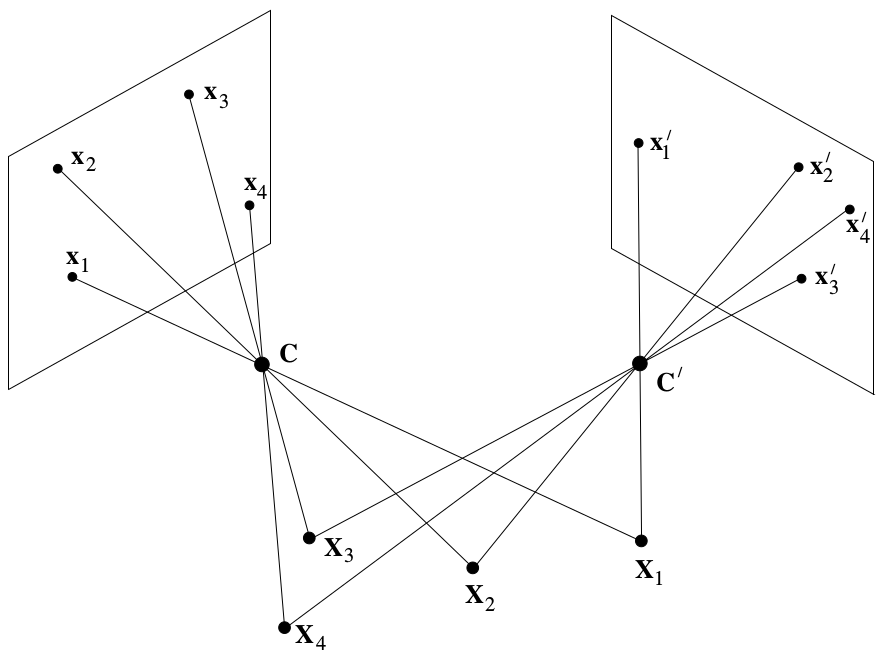
\includegraphics[width=.45\textwidth]{planos2}}\hspace{5mm}%}
	\subfigure[]{\label{fig:b}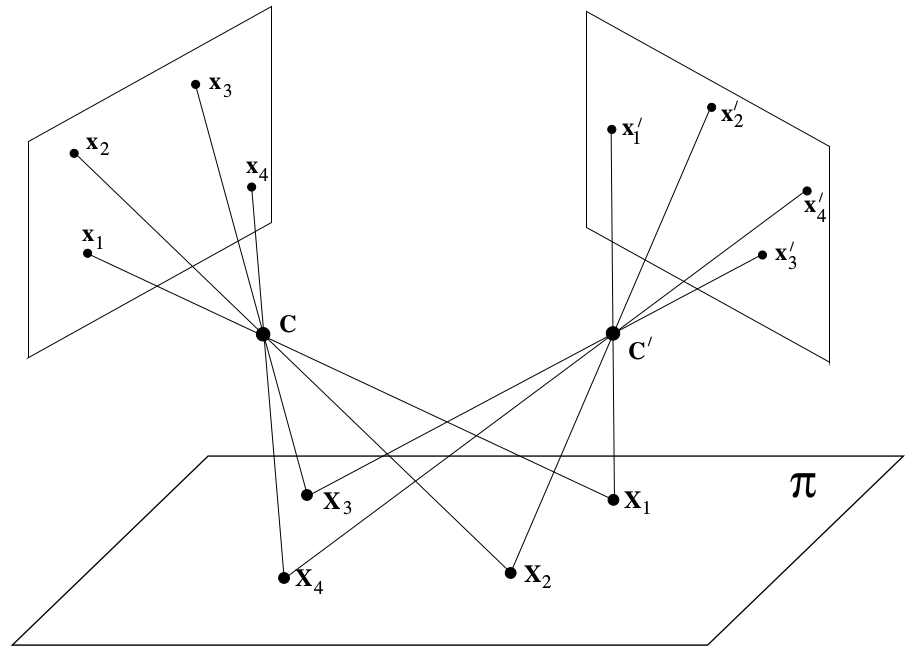
\includegraphics[width=.45\textwidth]{planos1}}
	\caption[Relacion de homografías]{Los puntos $\mathbf{C}$ y $\mathbf{C'}$ corresponden con los centros de la cámara en las distintas posiciones, Los puntos $\vec{x_i}$ y $\vec{x'_i}$ son la intersección de los puntos de la escena $\vec{X_i}$ en el plano de la imagen (formación de la imagen). Si la cámara se mueve no se podrá relacionar los planos de las imágenes con una homografía (izquierda), a menos que los puntos de la escena se encuentren todos en un mismo plano (derecha). Adaptado de \cite{zisserman}.}
	\label{imagen:planos}
\end{figure}

El primer paso para la estimación de la transformación consiste en encontrar 4 pares correspondientes de puntos, como cada punto en 2D posee 2-DoF ($x$ e $y$ del plano euclidiano de la imagen) con 4 puntos se tienen los 8-DoF. Luego por cada par de puntos se tienen (a partir de la ecuación \ref{matriz-perspectiva}) las siguientes relaciones: 
\begin{displaymath}
x'_i = \frac{x'}{w} = \frac{h_{11}x_i+h_{12}y_i+h_{13}}{h_{31}x_i+h_{32}y_i+h_{33}}, \qquad y'_i = \frac{y'}{w} = \frac{h_{21}x_i+h_{22}y_i+h_{23}}{h_{31}x_i+h_{32}y_i+h_{33}}
\end{displaymath}
Como se observa cada par de puntos genera dos ecuaciones lineales, mostradas a continuación luego de simplificar:
\begin{displaymath}
{x'_i ( h_{31}x_i+h_{32}y_i+h_{33} ) = h_{11}x_i+h_{12}y_i+h_{13}}
\end{displaymath}
\begin{displaymath}
{y'_i ( h_{31}x_i+h_{32}y_i+h_{33} ) = h_{21}x_i+h_{22}y_i+h_{23}}
\end{displaymath}
Escrito en forma matricial se puede expresar de la siguiente forma:
\begin{displaymath}
\mathtt{A}_i\vec{h}=\vec{0}
\end{displaymath}
Donde 
\begin{displaymath}
\mathtt{A}_i =
\begin{bmatrix}
-x_i&-y_i&-1&0&0&0&x'_ix_i&x'_iy_i&x'_i\\
0&0&0&-x_i&-y_i&-1&y'_ix_i&y_i'y_i&y'_i
\end{bmatrix}
\end{displaymath}
Y
\begin{displaymath}
\vec{h}^\mathtt{T} = (h_{11},\, h_{12},\, h_{13},\, h_{21},\, h_{22},\, h_{23},\, h_{31},\, h_{32},\, h_{33})
\end{displaymath}
Dado que 1 pareja arroja 2 ecuaciones lineales, 4 parejas arrojarían 8 ecuaciones, y se puede resolver el sistema para un factor multiplicativo dado por $h_{33}$ ($h_{33}=1$). La única restricción que tiene esta sistema de ecuaciones para asegurar un resultado único, es que no se tengan 3 puntos que residan en la misma linea. Con esto se tiene el siguiente sistema de ecuaciones:
\begin{displaymath}
\mathtt{A}\vec{h}=
\begin{bmatrix}
-x_1&-y_1&-1&0&0&0&x'_1x_1&x'_1y_1&x'_1\\
0&0&0&-x_1&-y_1&-1&y'_1x_1&y_1'y_1&y'_1\\
-x_2&-y_2&-1&0&0&0&x'_2x_2&x'_2y_2&x'_2\\
0&0&0&-x_2&-y_2&-1&y'_2x_2&y_2'y_2&y'_2\\
-x_3&-y_3&-1&0&0&0&x'_3x_3&x'_3y_3&x'_3\\
0&0&0&-x_3&-y_3&-1&y'_3x_3&y_3'y_3&y'_3\\
-x_4&-y_4&-1&0&0&0&x'_1x_1&x'_1y_1&x'_4\\
0&0&0&-x_4&-y_4&-1&y'_4x_4&y_4'y_4&y'_4
\end{bmatrix}
\begin{bmatrix}
h_{11}\\h_{12}\\h_{13}\\h_{21}\\h_{22}\\h_{23}\\h_{31}\\h_{32}\\h_{33}
\end{bmatrix}
= 0
\end{displaymath}
Añadiendo la condición de 	 $\left | \mathtt{H} \right | = 1$ para evitar la solución trivial $\vec{h}=0$. Luego se puede resolver mediante el método de descomposición en valores singulares SVD (del inglés: Singular Value Decomposition) con $\mathtt{A} = \mathtt{U}\mathtt{S}\mathtt{V}^\mathtt{T}$, donde $\mathtt{U}$ y $\mathtt{V}$ son matrices ortogonales; y $\mathtt{S}$ es una matriz formada con los valores singulares de $\mathtt{A}$ en su diagonal principal, ordenados en orden descendente. Finalmente el vector singular unitario correspondiente con el menor valor singular es la solución $\vec{h}$.

En este punto, la matriz encontrada se puede usar para transformar $\vec{x} \to \vec{x'}$, o bien se puede usar la inversa ($\mathtt{H^{-1}}$) para realizar el mapeo en sentido contrario.

Dada la naturaleza no plana de las escenas del mundo real, o bien debido a la inexactitud al medir los puntos cuando se captura una imagen, es muy poco probable que los puntos correspondientes residan en un mismo plano. Por otra parte es muy común que para aplicaciones de mapeo automático se cuenten con una gran cantidad de puntos correspondientes, con lo cual se tiene un sistema sobre determinado. En este caso es necesario realizar aproximaciones que permitan encontrar ya no la única homografía, sino la mejor, en función a los datos con los que se cuenten. Para esto es usual el uso de algoritmos que estiman la matriz buscando minimizar alguna función de costo.

Uno de los algoritmos mas usados para encontrar el mejor modelo está basado en el método RANSAC (del inglés: Random Sample Consensus), el cual es explicado a continuación.

%%%%%%%%%%%%%%%%%%%%%%%%%%%%%%%%%%%%%%%%%%%%%%%%%%%%%%%%%%
\subsubsection*{RANSAC}

Éste es un método iterativo que permite calcular los parámetros de un modelo, a partir de un conjunto de datos que presentan valores atípicos. En nuestro caso, se tiene un conjunto sobre determinado de pares de puntos correspondientes, de los cuales se deben seleccionar los mejores 4 pares para estimar la mejor matriz de transformación, siendo la mejor aquella que logre minimizar la función de costo planteada.


Como ya se ha mencionado, las escenas que se estudian no son completamente planas, lo que provoca una inexactitud al estimar la transformación. Para lograr establecer un modelo, el método RANSAC considera solo los mejores datos que se logren ajustar a él, en este sentido se definen los \textit{inliers} y \textit{outliers}, donde los \textit{inliers} son aquellos valores que logran encajar en el modelo deseado, mientras que los \textit{outliers} son aquellos que no logran hacerlo. Por ejemplo: si se tienen un conjunto de puntos cuya distribución corresponden con el plano del suelo, estos serian los \textit{inliers}, y por otro lado aquellos puntos que no pertenecen a este plano serian los \textit{outliers}, ya sea por un emparejamiento erróneo o que pertenezcan a un segmento de distinta altitud de la escena. En la figura \ref{imagen:ransac} se ilustra esta distinción.

\begin{figure}[h]
	\centering
	\includegraphics[width=14cm]{ransac.pdf}
	\caption[Mejor modelo - RANSAC]{Representación de un plano visto lateralmente. Los puntos amarillos corresponden con los utilizados para establecer el modelo (para calcular la matriz). Los puntos azules corresponden con los \textit{inliers}, mientras que los rojos con los \textit{outliers}. La distancia para la función de coste se mide desde cada punto hasta el plano modelo, considerando únicamente los \textit{inliers}.}
	\label{imagen:ransac}
\end{figure}

Ahora bien es necesario establecer la función de costo que buscará minimizar el algoritmo. En este caso se intenta disminuir el error cuadrático medio, donde el error es medido con la distancia de los puntos (inliers) correspondientes. Tal y como se observa en la figura \ref{imagen:ransac} el método RANSAC establece un perímetro que le permite distinguir \textit{inliers} de \textit{outliers}, ahora bien una vez se logran distinguir, el algoritmo solo considera los mejores para obtener el costo o peso asociado al modelo estimado, calculando para esto la distancia desde cada inlier hasta el plano. Este proceso se puede apreciar en el algoritmo \ref{ransac}.

\begin{figure}[hb]
	\centering
	\begin{minipage}{\linewidth}
		\begin{algorithm}[H] %or another one check
			\caption{Estimación de matriz de transformación RANSAC}
			\label{ransac}
			\SetAlgoLined
			\Begin{
				\While{No se llegue al maximo de iteraciones}
				{
					Se toman 4 parejas correspondientes\;
					Se calcula la matriz de homografía\;
					Se aplica la matriz sobre los puntos de origen\;
					Se calcula el error basado en distancia\tcp*{Solo considerando \textit{inliers}}
					\If{Error $<$ MejorError}
					{
						Guardar matriz como la mejor\;
						Guardar Error como el mejor\;
					}
				}
			}
		\end{algorithm}
	\end{minipage}
\end{figure}



%%%%%%%%%%%%%%%%%%%%%%%%%%%%%%%%%%%%%%%%%%%%%%%%%%%%%%%%%%
\section{Generación de sub-mosaicos}

El proceso mas simple para la generación de un mosaico consiste en añadir imágenes siguiendo los procesos planteados previamente, estableciendo el registro, y luego aplicando la matriz de transformación para lograr referenciarlas en el plano del mosaico. Ahora bien, para el caso del primer par de imágenes, esta practica implica que se halló la transformación desde la nueva añadida hacia la primera, tomando esta primera como plano de referencia. Esto se conoce como el proceso básico para la elaboración de mosaicos, en el cual se considera la primera imagen como referencia global para la construcción del mapa. La selección errónea de una imagen de referencia puede generar grandes distorsiones en el mosaico (especialmente para mapas grandes), y considerando el sistema simple, si no se cuenta con una primera imagen que se encuentre muy bien alineada con el plano del suelo, se comprometerá gravemente el resultado final del mosaico.

En busca de resolver este problema, \textit{Bellavia et. al.} en \cite{bellavia-ref,bellavia-ransac} plantean el modelo de sub mosaicos para lograr reducir el error geométrico producto de la mala selección de la imagen de referencia. Este sistema propone una estrategia para la selección del mejor plano de referencia que logre minimizar el error de distorsión, mediante la construcción de pequeños segmentos de mosaico que se alinean bajo el esquema básico, pero que poseen localmente poca distorsión geométrica.

\begin{figure}[h]
	\centering
	\includegraphics[width=0.6\linewidth]{submosaico.pdf}
	\caption[Generación de sub mosaicos]{Los cuadros verde y rojo son dos sub mosaico temporalmente continuos. El cuadro amarillo se convierte en el rojo relleno por presentar mucha distorsión.}
	\label{imagen:generacion-submosaico}
\end{figure}

La generación de los sub mosaicos consiste en el siguiente proceso: refiriéndonos a la figura \ref{imagen:generacion-submosaico}, se selecciona como referencia la primera imagen (cuadro verde relleno), se añaden imágenes al sub mosaico sucesivamente hasta que la siguiente presente mucha distorsión (cuadro amarillo), en este punto se crea un nuevo sub mosaico (cuadros rojos) y se añade aquella que presentó mucha distorsión como referencia para el nuevo sub mosaico. Donde el error es medido en función al área y el cociente entre semi-diagonales.

Siguiendo este proceso se van construyendo sub mosaicos hasta que no se cuenten con mas imágenes. Una vez se han creado todos los sub-mosaicos es necesario unirlos. En este punto cada sub mosaico considera la primera imagen como el plano de referencia, por lo tanto es necesario definir cual será la referencia bajo la cual éstos deben unirse. Para esto se utiliza la homografía que logre disminuir el error de distorsión sobre todos las imágenes del sub mosaico, esta transformación se define como \textit{homografía promedio}. El proceso para su obtención se detalla a continuación.



\subsection{Matriz de transformación promedio}\label{seccion-hpromedio}



Para encontrar la homografía promedio se aplica un algoritmo basado en el método RANSAC, el cual consiste en obtener 4 pares de puntos correspondientes ($x^1_i   \leftrightarrow x^2_i$) entre los dos sub mosaicos (verde y rojo) para un número fijo de iteraciones, seguidamente para dichos puntos se calcula el punto medio ($x^a_i$), luego se calcula la matriz que transforma los puntos del primer sub mosaico hacia los puntos medios ($x^a = \mathtt{H}x^1$), después se aplica la homografía en el primer sub mosaico y se obtiene la distorsión para dicha transformación. Finalmente la matriz que logre minimizar la distorsión global en el nuevo sub mosaico es seleccionada como la homografía promedio. Éste proceso se muestra mejor estructurado en el algoritmo \ref{homografia-promedio}.


\begin{spacing}{0.8}
	\begin{algorithm}[h] %or another one check
		\caption{Calculo de matriz de homografia promedio}
		\label{homografia-promedio}
		\SetAlgoLined
		\Begin{
			\While{no se alcanza el maximo de iteraciones}{
				Seleccionar 4 puntos aleatorios del primer sub-mosaico\;
				Seleccionar los 4 puntos correspondientes en el segundo sub-mosaico\;
				Salcular el punto medio para cada par de puntos correspondientes\;
				Calcular la transformacion desde los puntos del primer sub-mosaico hasta los puntos medios\;
				Aplicar transformacion en el primer sub-mosaico\;
				Calcular error de distorsión en el primer sub-mosaico\;
				\eIf{el error es menor que el mas bajo obtenido}{
					Guardar el error como el mas bajo\;
					Guardar la matriz de transformación como la mejor\;
				}{
				Restaurar valores del primer sub-mosaico\;
			}	
		}
		Aplicar mejor matriz al primer sub-mosaico\;
	}
\end{algorithm}
\end{spacing}

El criterio para determinar el grado de distorsión de la imagen se observa en la ecuación \ref{eq-error}, tal y como se propone en \cite{bellavia-ref}:

\begin{equation}
E = \max\limits_{I_i\in S_j\cap S_k} (E^O + E^C + E^A + E^\alpha)
\label{eq-error}
\end{equation}


Siendo $I_i$ una imagen perteneciente al par de sub mosaicos $S_j,S_k$; con lo cual se considera la imagen que presente mas distorsión en el sub mosaico que se intenta unir. El error de cada tipo de error se encuentra normalizado en el rango $0\to 1$. 

$E^O$ mide el error sobre lados opuestos de la imagen.
\begin{equation}
E^O = 1 - \frac{1}{2}  \left(  \frac{\min (l_1, l_3)}{\max (l_1, l_3)} +  \frac{\min (l_2, l_4)}{\max (l_2, l_4)} \right)
\end{equation}

$E^C$ mide el error sobre lados consecutivos, siendo $m > n$.
\begin{equation}
E^C = 1 - \frac{\min (r, \frac{m}{n})}{\max (r, \frac{m}{n})}
\end{equation}

Donde $r$ es el mínimo cociente entre lados consecutivos, expresado como:
\begin{displaymath}
r = \left( \frac{l_1}{l_2},\, \frac{l_2}{l_3},\, \frac{l_3}{l_4},\, \frac{l_4}{l_1} \right)
\end{displaymath}

$E^A$ mide el error del área
\begin{equation}
E^A = 1 - \frac{\min (A_{\tilde{I}_k},\, mn)}{\max (A_{\tilde{I}_k},\, mn)}
\end{equation}

$E^\alpha$ mide el error sobre los ángulos internos. 
\begin{equation}
E^\alpha = (\max (\cos\alpha_{12},\, \cos\alpha_{23},\, \cos\alpha_{34},\, \cos\alpha_{41}))^5
\end{equation}


\subsection{Selección de puntos característicos}\label{seleccion-grid}

Según se estudió en el método RANSAC, la estimación de una buena homografía depende de la distribución de los puntos en la escena. Es posible contar con una gran cantidad de puntos extraídos y emparejados en una sección de la escena que no corresponde con el mejor modelo del plano de ésta, lo que indica que la matriz de homografía se ajuste a dicha región por ofrecer menor peso en la función de coste. En cambio, el resultado esperado es que se tenga una mejor distribución de puntos en la escena de modo que se tenga una ponderación de igual magnitud para todas las regiones del suelo.


\subsection{Seguimiento de puntos}\label{seguimiento-puntos}

Ya hemos visto el proceso simple de relacionar dos imágenes, donde luego de aplicar la transformación a la nueva imagen, ésta presentará cierto nivel de distorsión, afectando que las imágenes siguientes logren establecer una relación robusta de puntos.

La primera propuesta consiste en buscar parejas de puntos correspondientes entre la nueva imagen y el mosaico (todas las imágenes añadidas previamente), pero esto trae consigo un alto costo computacional cuando se cuenta con un mosaico de gran tamaño. A pesar de que se puede restringir el área de búsqueda hacia el mínimo cuadro que encierra la ultima imagen transformada, el efecto de distorsión mencionado afecta la detección e identificación de puntos correspondientes.

\begin{figure}[h]
	\centering     %%% not \center
	\subfigure[]{\label{fig:ec-a}\includegraphics[width=.7\textwidth]{track1.pdf}}
	
	\subfigure[]{\label{fig:ec-b}\includegraphics[width=.5\textwidth]{track2.pdf}}
	
	\caption[Seguimiento de puntos]{Seguimiento de puntos. En (a) se realiza la extracción y emparejamiento en las imágenes originales, luego los puntos detectados en la imagen (2) son transformados por la homografía que ubica esa imagen en el mosaico. finalmente en (b) se halla la matriz de transformación para la nueva imagen usando la nueva correspondencia.}
	\label{imagen:track}
\end{figure}

Para solucionar este problema se propone realizar una extracción de puntos característicos para todas las imágenes en su versión original, y una vez se conozca la matriz de transformación que ubica una imagen en el mosaico. De igual forma se puede transformar la ubicación de los puntos detectados hacia la nueva ubicación. Este proceso se encuentra ilustrado en la figura \ref{imagen:track}.

Definiendo $\vec{x}^1_i$ como los puntos que corresponden a la nueva imagen, $\vec{x}^2_i$ como los que corresponden a la última añadida con sus dimensiones y posición original, y $\vec{x}^{2*}_i$ serian aquellos de la ubicación en el mosaico. Primero se realiza la detección para encontrar la correspondencia $\vec{x}^1_i \leftrightarrow \vec{x}^2_i$, luego se transforman los puntos $x^2_i$ a su ubicación correspondiente en el mosaico $x^{2*} = \mathtt{H}^*\vec{x}^2$ ($\mathtt{H}^*$ conocida). Finalmente se encuentra la matriz de transformación para la nueva imagen con la siguiente relación: $\vec{x}^{2*} = \mathtt{H}\vec{x}^1$.



\subsection{Relación con vecinos}\label{seccion-vecinos}

Tal y como se ha planteado hasta este punto, el proceso de registro consiste establecer relación entre dos imágenes para estimar la homografía que permite alinearla. Esta practica es ideal cuando se tiene un movimiento continuo del robot al explorar el suelo, o bien cuando se tiene un bajo porcentaje de superposición (ver figu, con lo cual se dificulta que una tercera imagen se relacione con la primera. Por otro lado, cuando estas condiciones no se cumplen, es necesario plantear soluciones que aprovechen toda la información posible de las imágenes para tener un sistema mucho mas robusto. En base a esto se planteó una técnica de búsqueda por vecinos para mejorar la etapa de registro, el proceso consiste en buscar relaciones de puntos entre imágenes que no sean temporalmente continuas, es decir, intentar relacionar una imagen con un grupo de todas aquellas inmediatamente anteriores, y que tengan información en común (intersección), a las cuales llamaremos imágenes vecinas (ver figura).





%%%%%%%%%%%%%%%%%%%%%%%%%%%%%%%%%%%%%%%%%%%%%%%%%%%%%%%%%%%%%%%%%%%%%%%%
\section{Corrección euclidiana}\label{seccion-ec}

La concatenación de un gran grupo de imágenes en la formación de un mosaico, suele traer consigo un error de distorsión acumulado producto de la estimación de la mejor matriz de homografía, afectando en muchos casos el tamaño original de las imágenes. Para resolver este problema \textit{A. Elibol y R. Garcia} en \cite{elibol} proponen un método de corrección global basado en transformaciones de isometría.

Considerando que un robot de exploración (aéreo o submarino) con una cámara dirigida hacia abajo presenta pocas variaciones de rotación (ángulo de cabeceo y balanceo), además de intentar mantener una altura constante con el suelo, las transformaciones que describan su movimiento debería estar descrita por esos grados de libertad (rotación y translación, sin escala). En este sentido, se utiliza un modelo del sub mosaico que utiliza solamente transformaciones de isometría (ecuación \ref{matriz-isometria}). Así mismo, al no contar con datos de navegación, como GPS que no está presente en aplicaciones bajo el agua, el método propuesto presenta una buena aproximación para reducir el error de tamaño en las imágenes del extremo del mosaico. Este proceso se encuentra listado a continuación, además se ilustra 

\begin{enumerate}%for capital roman numbers.
	\item Alinear imágenes usando transformaciones de Isometría
	\item Seleccionar coordenadas del borde del mosaico
	\item Alinear imágenes usando transformaciones de perspectiva
	\item Seleccionar mismas coordenadas del paso (2)
	\item Hallar homografía desde desde los puntos (2) hasta (4)
	\item Aplicar transformación a todas las imágenes del mosaico.
\end{enumerate}

Con respecto  a la selección de los puntos frontera del mosaico, el primer par se selecciona considerando aquellos de la primera imagen que se encuentren mas alejados del centro de la última, y para el ultimo par se consideran aquellos de la última imagen mas alejados del centro de la primera.

\section{Resultados}

En esta sección se presentan los resultados de aplicar 
\section{Resumen}

En este capítulo se describieron los principios básicos que permiten alinear imágenes bajo un mismo sistema de referencia, utilizando la información que proveen los extractores de características locales. Para esto se introdujeron los distintos niveles de transformaciones geométricas en base a los grados de libertad que ofrece cada una y a la cantidad de variables que preservan de las imágenes, además del proceso para su obtención.

Luego se introdujeron los diversos problemas que se tienen al realizar la alineación bajo el esquema mas simple. En función a esto se buscó resolver errores producidos por la mala selección de la imagen de referencia, por realizar el registro con las imágenes deformadas, y por considerar únicamente la ultima imagen añadida para establecer la referencia necesaria.

Finalmente se presentaron los resultados que validan los métodos descritos, obteniendo de estos mejoras claras sobre la geometría del mosaico y la robustez para su construcción.


